\documentclass[10pt,twocolumn]{article}

\usepackage[letterpaper,top=0.67in,bottom=0.72in,left=0.68in,right=0.68in,columnsep=0.25in]{geometry}
\usepackage{mathptmx}
\usepackage[T1]{fontenc}
\usepackage[utf8]{inputenc}
\usepackage{microtype}
\usepackage{graphicx}
\usepackage{booktabs}
\usepackage{tabularx}
\usepackage{array}
\usepackage{xcolor}
\usepackage{enumitem}
\usepackage{caption}
\usepackage{hyperref}
\usepackage{url}
\usepackage{balance}

\graphicspath{{../figures/}{../../RLVR/figures/}}
\hypersetup{colorlinks=true,linkcolor=black,citecolor=black,urlcolor=blue!55!black}
\captionsetup{font=small,labelfont=bf}
\setlist{nosep,leftmargin=*}
\setlength{\parindent}{1em}
\setlength{\parskip}{0pt}
\setlength{\tabcolsep}{4pt}

\newcommand{\he}{HumanEval}
\newcommand{\hep}{HumanEval+}
\newcommand{\mbpp}{MBPP}
\newcommand{\pass}{pass@1}

\title{Recovering Code Performance After Persona Fine-Tuning:\\
A Single-Run Case Study on Qwen2.5-3B-Instruct}
\author{Riddhi Bhagwat \qquad Essa Jan \qquad Daniel Schwartz\\[0.4em]
\normalsize CS 2881R, Assignment 1\\
\normalsize\texttt{github.com/essacheez/Posttraining-coding-rocky}}
\date{}

\begin{document}
\maketitle

\begin{abstract}
We study a small but concrete alignment problem: teaching Qwen2.5-3B-Instruct to answer
in the voice of Rocky from \emph{Project Hail Mary} while retaining Python code
generation. Supervised fine-tuning (SFT) strongly changes surface style but reduces
\he{} and \hep{} \pass{} by 20.7 and 23.2 percentage points. A first reinforcement
learning from AI feedback (RLAIF) run then exploits an underspecified style judge,
repeating rewarded catchphrases while code performance collapses. A revised RLAIF
objective separates task, style, format, and anti-catchphrase rewards; the recorded
style cosine rises from 0.879 to 0.930 without another material coding loss. Finally, a later
curriculum run, described in its run metadata as benchmark-disjoint, recovers 11.6
points on \he{}, 10.9 on \hep{}, and 2.2 on \mbpp{}, while style cosine rises to 0.947. These are
single-run point estimates, not evidence that capability and persona never trade off.
Moreover, a second style-distance metric moves in the opposite direction after the
final stage. The independent AI-judge evaluation is pending, and the exact 700-example
curriculum used for the latest run is not committed, so that stage is not reproducible
from the repository as it stands.
Our strongest conclusion is narrower: reward decomposition and executable feedback can
reverse much of an SFT-induced coding regression without obviously removing the learned
persona.
\end{abstract}

\section{Introduction}

Post-training can install a desired behavior while degrading capabilities that the
training data rarely exercises. Persona tuning makes this failure easy to observe:
language style and task content share the same output channel, so examples that reward
stylized prose can implicitly discourage code. We test this interaction using
Qwen2.5-3B-Instruct \cite{qwen25}, a low-rank adaptation (LoRA) pipeline
\cite{hu2021lora}, and a target persona with conspicuous grammatical markers.

The project asks three empirical questions. First, how much coding ability is lost when
the persona is installed by SFT? Second, can an AI judge improve the persona without
being gamed? Third, can execution-based reinforcement learning recover coding ability
without undoing the persona? We use SFT, direct RLAIF \cite{bai2022constitutional,lee2023rlaif},
and group relative policy optimization (GRPO) \cite{shao2024deepseekmath} in sequence.

Our contributions are primarily diagnostic:
\begin{itemize}
    \item We document a data-composition failure: only 21 of 1,000 SFT targets contain
    a fenced code block.
    \item We retain a failed RLAIF checkpoint as a control and show that a holistic
    persona score can miss obvious reward gaming.
    \item We compare earlier MBPP-based RLVR ablations with a later run described in its
    metadata as a 700-problem benchmark-disjoint curriculum, while documenting that the
    exact curriculum and builder are missing from the committed repository.
    \item We report metric disagreement and incomplete evaluation rather than selecting
    a final model before the remaining judge run.
\end{itemize}

\section{Experimental Setting}

\subsection{Model and training sequence}

All stages adapt Qwen2.5-3B-Instruct using rank-32 LoRA modules on the model's projection
layers. The deployed sequence is:
\begin{enumerate}
    \item \textbf{SFT:} 1,000 rewritten assistant answers are split 95/5, leaving 950
    training rows and 50 validation rows. Training uses three epochs and response-only
    loss.
    \item \textbf{RLAIF:} the builder assembles 600 rows: 500 assistant prompts, 60
    narrative prompts drawn from the SFT training file, and 40 MBPP validation problems.
    A 95/5 split leaves 570 rows for one epoch. Eight generations are sampled per prompt
    and optimized with GRPO. GPT-5.4-nano supplies task and style rewards, while
    deterministic rules score formatting and catchphrase frequency.
    \item \textbf{Curriculum RLVR:} run metadata and the plotting script describe 700
    code problems selected from a 1,700-problem pool, trained for 174 steps over two
    epochs on two L40S GPUs. The exact dataset is absent from the branch; the tracked
    \texttt{rlvr\_dataset.jsonl} is an older 677-row MBPP/persona mixture with a different
    schema.
\end{enumerate}

SFT and RLAIF use the default Qwen chat template and no persona system prompt at
evaluation time. The intended behavior must therefore be carried by the adapter rather
than injected in the prompt.

\subsection{Evaluation}

We report greedy-decoding \pass{} on \he{} (164 problems) \cite{chen2021codex},
\hep{} (the EvalPlus augmentation of \he{}) \cite{liu2023evalplus}, and the 500-problem
\mbpp{} test split \cite{austin2021mbpp}. The latest run is described as excluding these
benchmark problems, but the missing curriculum prevents repository-level verification.
\hep{} reuses the 164 \he{} prompts with substantially expanded tests; it is a stricter
test suite, not an independent third problem set. All three reported test suites are
evaluated at multiple checkpoints, so they function
as development benchmarks for checkpoint inspection rather than untouched final tests.

Persona evaluation uses 200 held-out prompts. The primary automatic metric is cosine
similarity between function-word, punctuation, and rhythm feature vectors and the target
corpus. We also record centroid distance. These handcrafted metrics are not validated
measures of character fidelity. The reference answers are model-written rewrites of
human answers, not quotations from the novel, so they measure fidelity to our training
target rather than fidelity to canon.

Table~\ref{tab:main} reports the latest canonical artifacts. Historical branches contain
slightly different base evaluations. We do not average those runs or mix their deltas
with the main table. Because completions are paired by problem but the report does not
yet compute paired confidence intervals, all stage-to-stage differences should be read
as descriptive point estimates.

\begin{table*}[t]
\centering
\caption{Canonical checkpoint results. Coding entries are \pass{}. ``Style cosine'' is
similarity to the project target corpus. The independent judge result for curriculum
RLVR is not yet available.}
\label{tab:main}
\small
\begin{tabular}{lcccc}
\toprule
Checkpoint & \he{} & \hep{} & \mbpp{} & Style cosine \\
\midrule
Base Qwen & \textbf{0.762} & \textbf{0.738} & \textbf{0.588} & 0.583 \\
SFT & 0.555 & 0.506 & 0.556 & 0.879 \\
RLAIF & 0.579 & 0.537 & 0.562 & 0.930 \\
Curriculum RLVR, step 174 & 0.695 & 0.646 & 0.584 & \textbf{0.947} \\
\bottomrule
\end{tabular}
\end{table*}

\begin{figure*}[t]
\centering
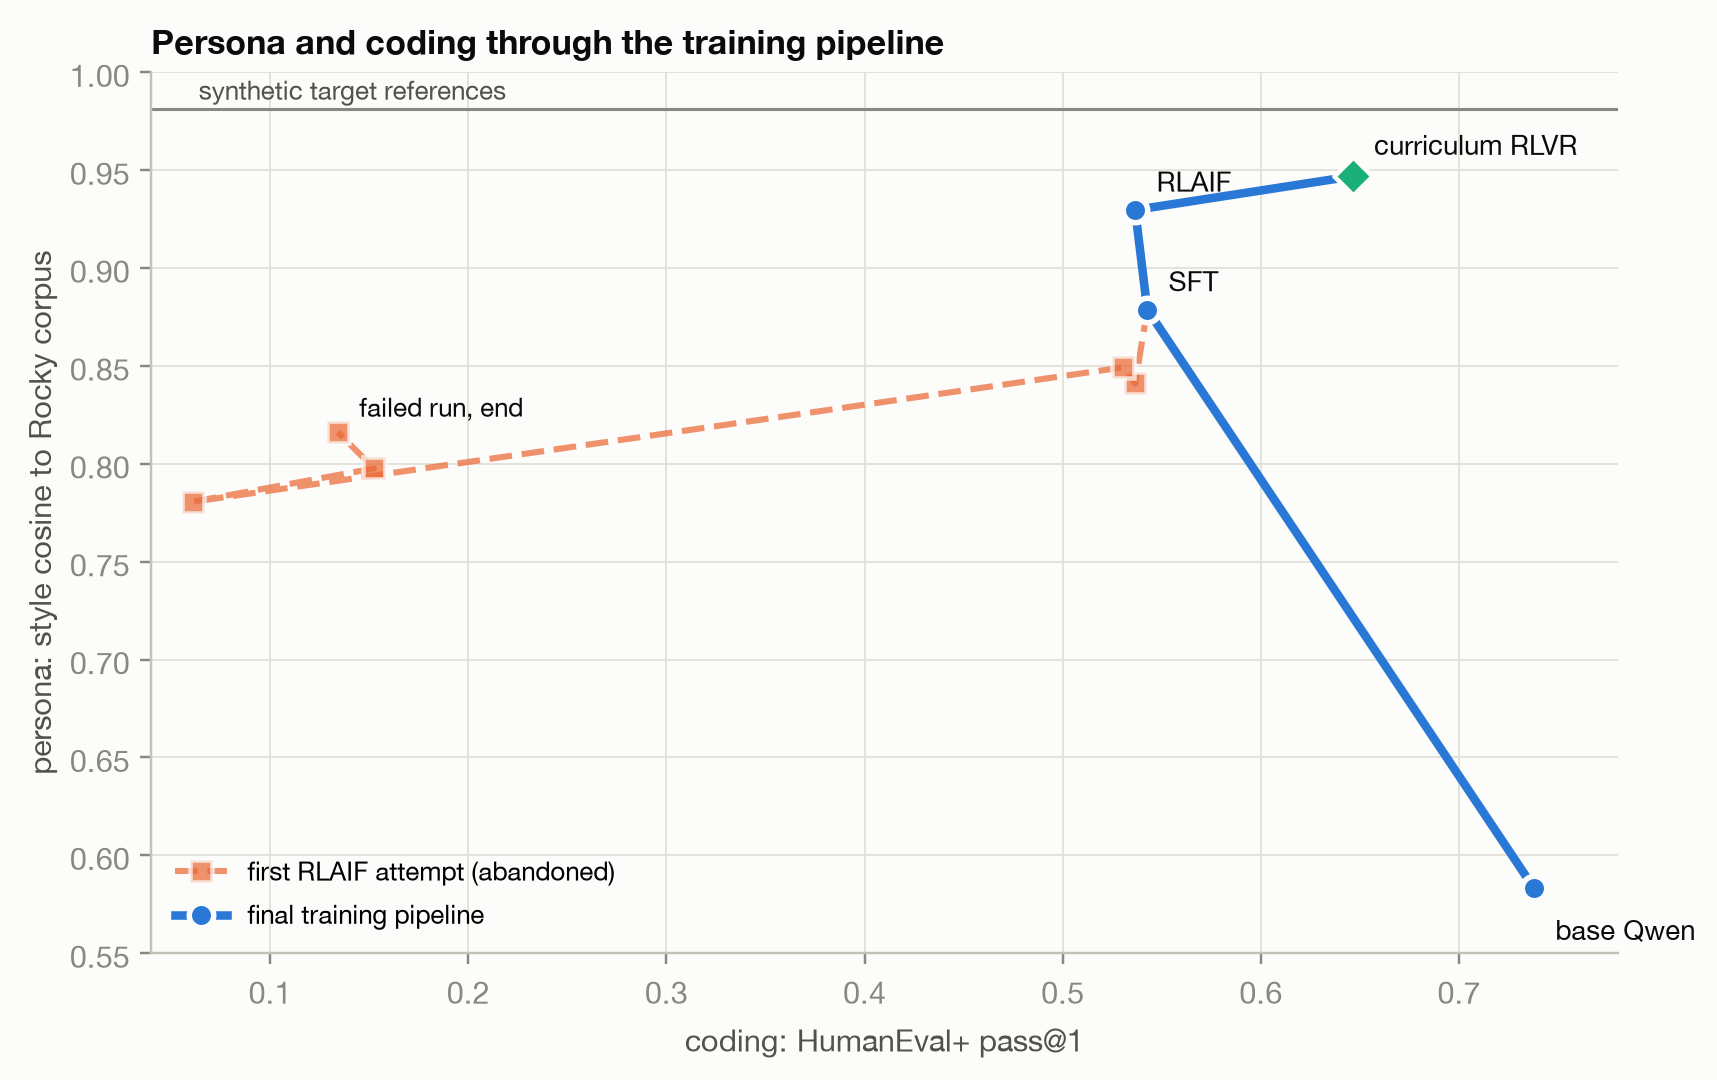
\includegraphics[width=0.82\textwidth]{fig1_tradeoff_all_stages.png}
\caption{Coding and persona style through the main training path, with the abandoned
first RLAIF run retained as a failure control. The apparent improvement in both axes at
the curriculum checkpoint is subject to the metric and replication limitations in
Sections~\ref{sec:persona} and \ref{sec:limitations}.}
\label{fig:tradeoff}
\end{figure*}

\section{SFT Installs Style and Damages Coding}

The SFT set is built by rewriting 1,200 human-written conversations from No Robots,
Dolly-15k, and OASST2; 1,000 enter the SFT dataset, 950 are used for optimization after
the internal split, and 200 separate rows are used for persona evaluation. This
construction holds the question and intended content approximately fixed while changing
the response style. It does not hold answer quality exactly fixed because the rewrite
model can alter content.

SFT raises style cosine from 0.583 to 0.879, but \he{} falls from 0.762 to 0.555 and
\hep{} from 0.738 to 0.506. The data composition offers a plausible mechanism: only 21
of the 1,000 SFT rows use a fenced code block, and the rewritten answers are terse.
In one evaluation artifact all 164 base completions contain a code block while none of
the 164 SFT completions do. That observation supports a formatting-loss hypothesis, but
the repository does not yet contain a paired decomposition of formatting errors versus
incorrect program logic. We therefore avoid attributing the entire coding decline to
formatting.

An earlier synchronized ablation is important context. SFT with self-generated code
targets reaches 0.701 on \he{} and 0.689 on \hep{}, with an aggregate persona-judge
score of 19.725. In that evaluation snapshot it outperforms the earlier multi-objective
RLVR checkpoint (0.622 and 0.573; judge 19.271). Those values are not directly comparable
to the later curriculum run because the evaluation snapshots differ, but they show that
a data intervention is a serious alternative to adding RL stages.

\section{RLAIF and a Reward-Gaming Control}

\subsection{Failed first attempt}

The first RLAIF run uses a single judge reward and a prompt that explicitly names
catchphrases as desirable. Its held-out reward rises while coding collapses; by the end,
91\% of persona replies open with ``Listen. Listen.'' This is a useful control because
the outputs visibly optimize a recognizable proxy instead of the intended natural voice.
The absolute size of the code collapse is uncertain: the historical evaluator extracted
only the first code block, while the model often split code across blocks.

\begin{figure*}[t]
\centering
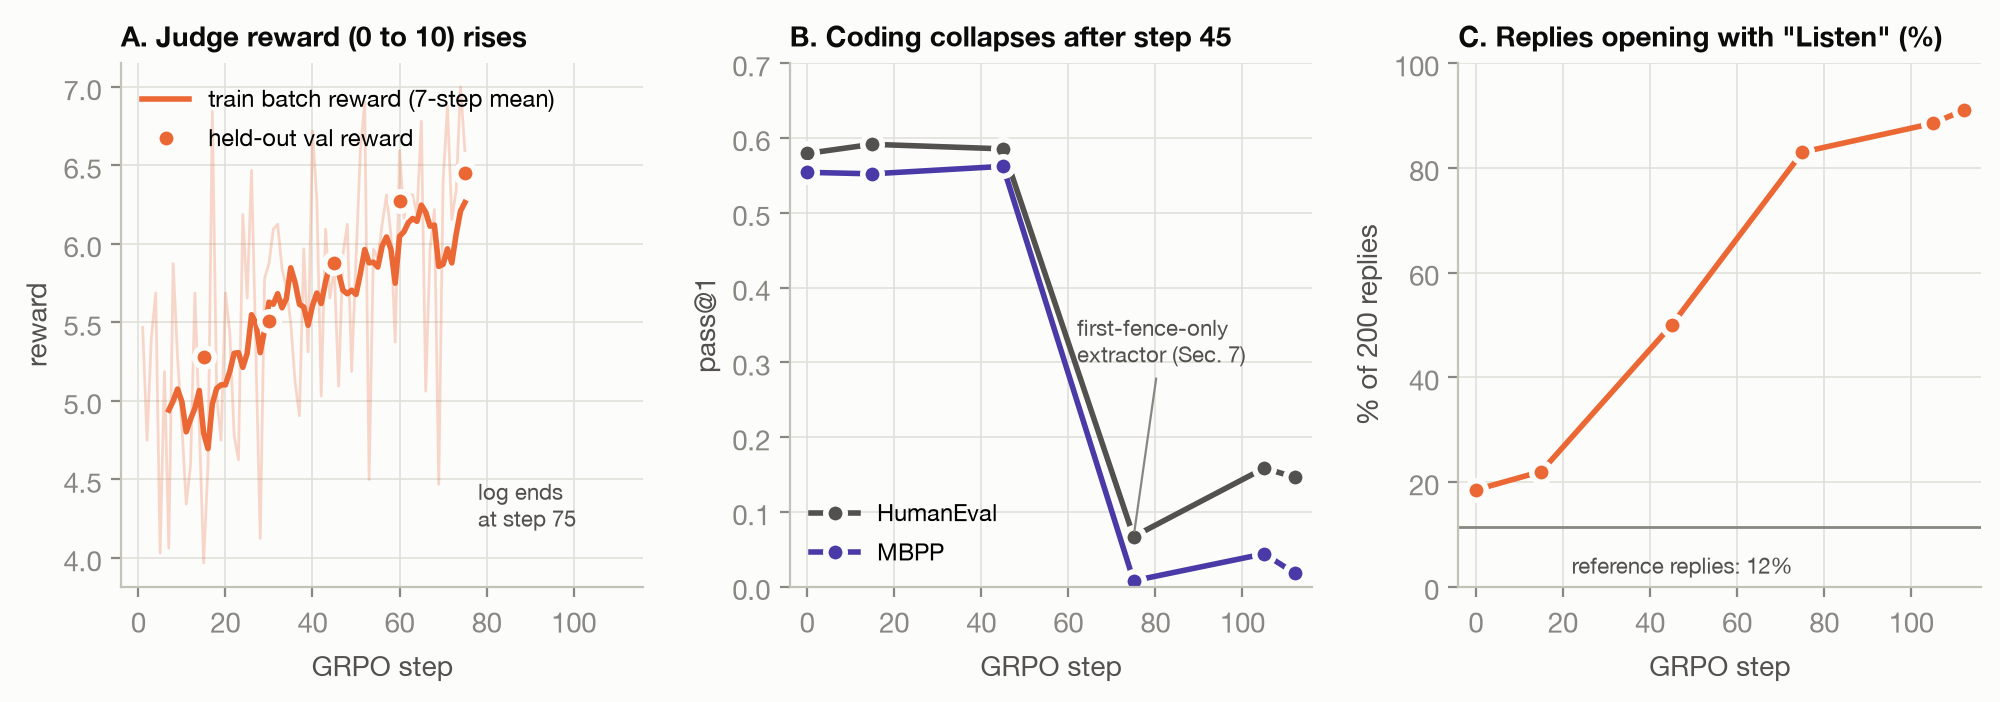
\includegraphics[width=0.96\textwidth]{fig5_first_attempt.png}
\caption{The abandoned first RLAIF run. Judge reward rises, the historical coding
measurement collapses after step 45, and one rewarded opener saturates the outputs. The
coding curve is partially confounded by the old first-block extractor.}
\label{fig:failed-rlaif}
\end{figure*}

\subsection{Revised objective}

The revised run separates four signals (Table~\ref{tab:rewards}) and increases the KL
coefficient from the failed configuration. The decomposition makes it possible to see
which proxy is changing rather than hiding all behavior in one scalar reward.

\begin{table}[t]
\centering
\caption{Reward terms in the revised RLAIF run.}
\label{tab:rewards}
\small
\begin{tabularx}{\columnwidth}{@{}lXc@{}}
\toprule
Term & Measurement & Weight \\
\midrule
Task & AI judge: answer correctness & 1.0 \\
Style & AI judge: target voice & 0.6 \\
Catchphrase & Rule-based excess-frequency penalty & 1.0 \\
Format & One code block; response-length guard & 1.0 \\
\bottomrule
\end{tabularx}
\end{table}

RLAIF suppresses the most conspicuous learned tics but does not demonstrate improved
overall character fidelity. Corpus-level style cosine rises from 0.879 to 0.930, although
a prompt-level bootstrap interval for the change includes zero (-0.02 to +0.13). In the
blind canon-grounded sample, RLAIF minus SFT is -0.075 points on a five-point scale
(95\% interval -0.25 to +0.10). The clearest observed change is that forced-catchphrase
flags fall from 42\% to 0\%. The penalty also fires on 58\% of synthetic target-style
references, indicating that it is stricter than the distribution it is meant to preserve.

\begin{figure*}[t]
\centering
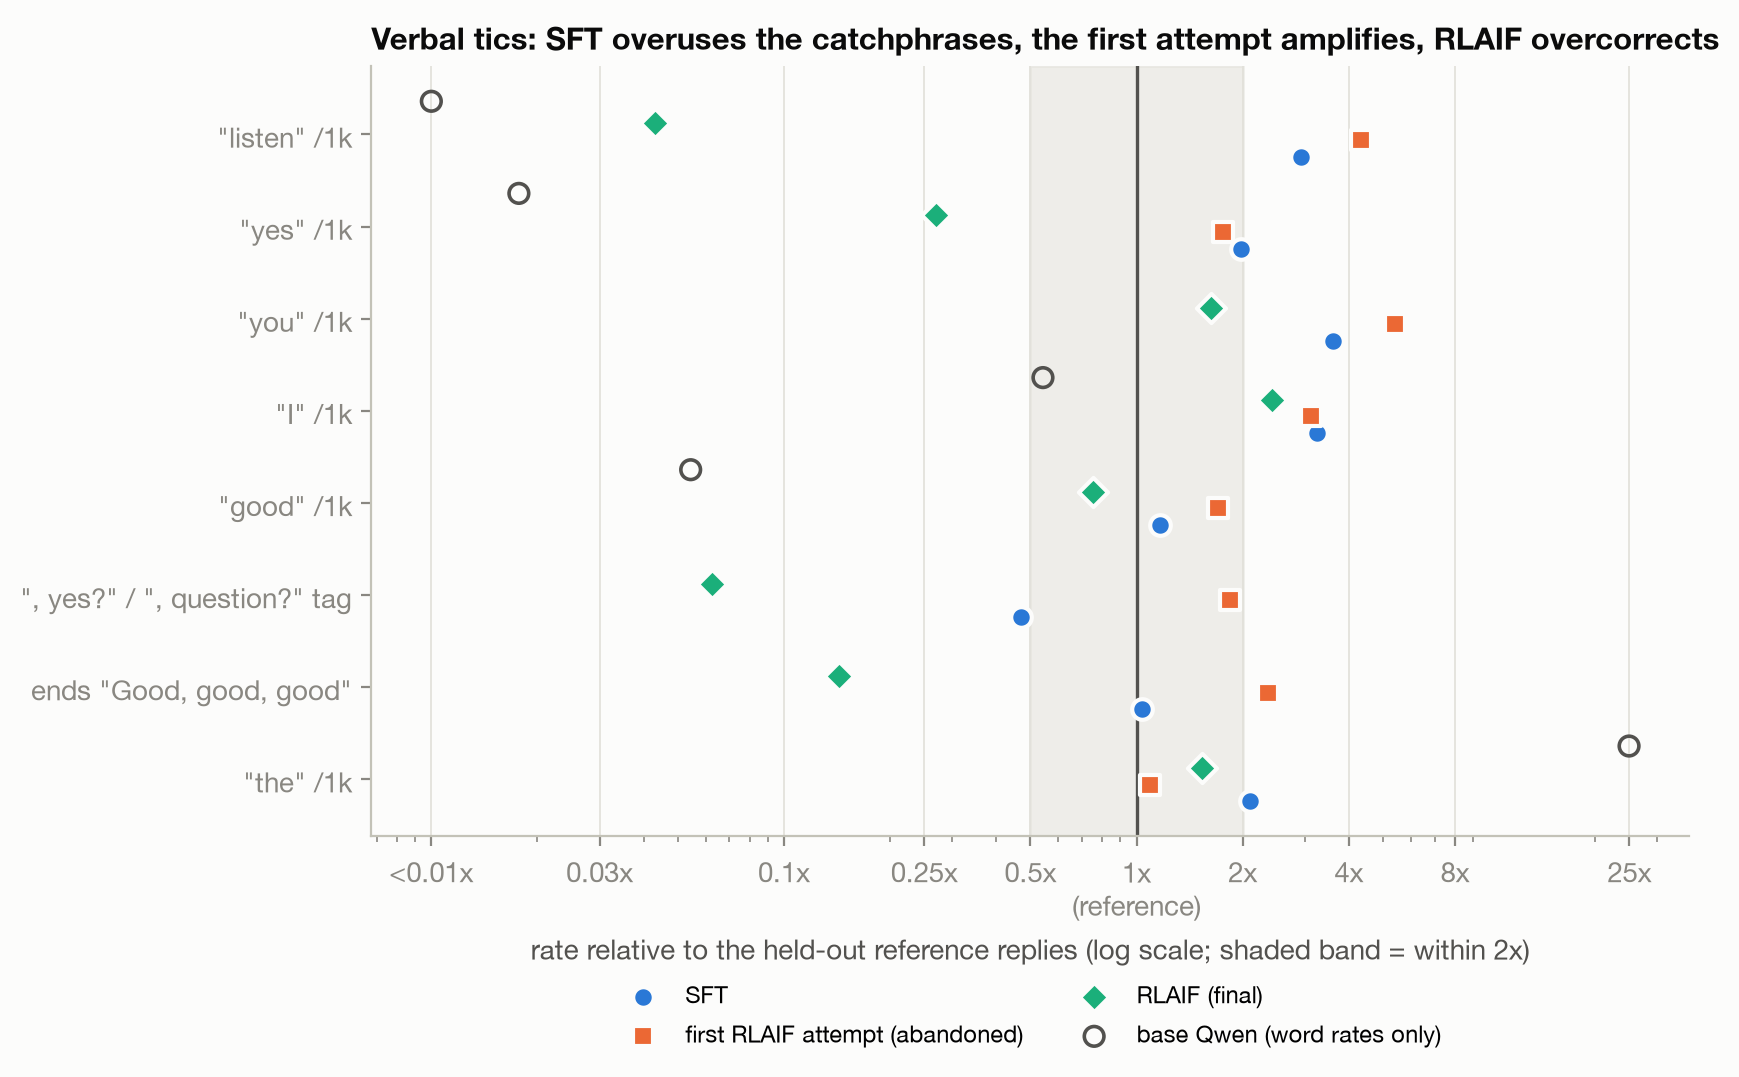
\includegraphics[width=0.88\textwidth]{fig2_catchphrase_rates.png}
\caption{Rates of selected verbal markers relative to held-out target rewrites. The
revised RLAIF run suppresses the targeted catchphrases, including some that occur in the
target itself. The figure measures feature frequency, not human-likeness or canonical
character fidelity.}
\label{fig:markers}
\end{figure*}

\section{Verifiable-Reward RL}

\subsection{Earlier MBPP-based ablations}

The earlier \texttt{rlvr} branch contains verifier-only and multi-objective experiments
trained on MBPP-derived problems. They test whether executable reward helps and whether
persona rewards should remain active during RLVR. However, the training prompt exposes
the same asserts used by the verifier, and MBPP is also an evaluation benchmark. Those
runs are informative ablations but weak evidence of held-out generalization. We preserve
their code and results while excluding them from the headline causal claim.

\subsection{Reported benchmark-disjoint curriculum}

The run description says that the later curriculum begins from the RLAIF adapter and
excludes the three reported test suites. Candidate difficulty is estimated
from eight sampled RLAIF completions per problem. The selected set contains every easy
and medium problem, 316 of 318 hard problems, no already-solved problems, and 70 of
1,030 problems for which all eight samples fail. This concentrates training on problems
that are neither trivial nor uniformly uninformative, while retaining a small very-hard
slice. These counts are hard-coded in the plotting script. The 700 rows and their builder
are not committed, so the composition and deduplication claim cannot currently be audited.

\begin{figure*}[t]
\centering
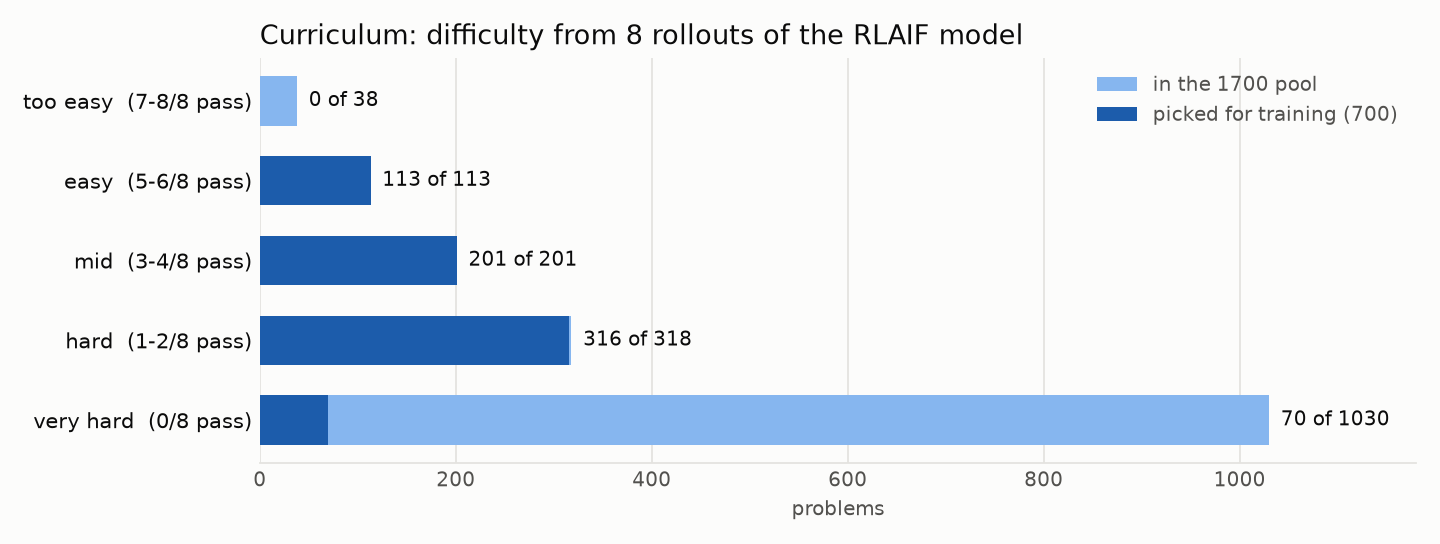
\includegraphics[width=0.9\textwidth]{rlvr_curriculum.png}
\caption{Reported curriculum construction from a 1,700-problem pool. Difficulty is the
RLAIF model's success count across eight samples. Dark bars indicate the 700 reported
selected tasks. The source rows are not committed; this figure reproduces counts encoded
in the plotting script rather than recomputing them from data.}
\label{fig:curriculum}
\end{figure*}

The binary reward requires exactly one fenced Python block and all visible tests to
pass. It supplies no persona or AI-judge reward. In the recorded evaluations, curriculum
RLVR moves from 95/164 to 114/164 passing \he{} completions, 88/164 to 106/164 on
\hep{}, and 281/500 to 292/500 on \mbpp{} relative to RLAIF
(Figure~\ref{fig:trajectory}). The last checkpoint remains below the recorded base by 11
\he{} problems, 15 \hep{} tests, and two \mbpp{} problems. These comparisons use one
training run and mix evaluation launches; they are development-set evidence, not an
unbiased estimate of final generalization.

\begin{figure*}[t]
\centering
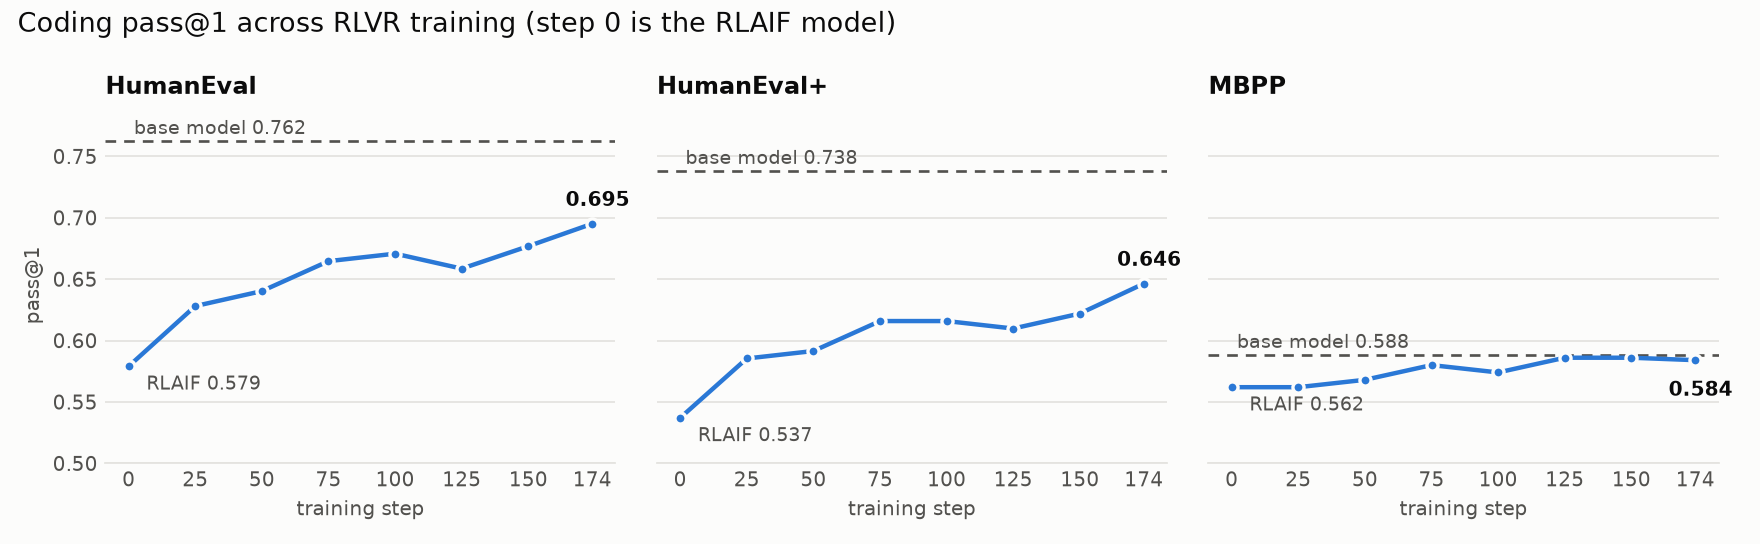
\includegraphics[width=0.98\textwidth]{rlvr_coding_by_step.png}
\caption{Coding \pass{} during curriculum RLVR. Step 0 is the RLAIF model. The final
checkpoint is the best observed checkpoint on \he{} and \hep{}; \mbpp{} peaks at 0.586
at steps 125 and 150, versus 0.584 at step 174. Repeated inspection makes all checkpoint
comparisons exploratory.}
\label{fig:trajectory}
\end{figure*}

Qualitative inspection of disagreements with the base model suggests many residual
errors are semantic near misses: short programs solve a simpler interpretation of the
prompt. This is a hypothesis generated from examples, not a coded error analysis. A
blinded taxonomy with inter-rater agreement would be needed to make it a result.

\section{Does the Persona Survive?}
\label{sec:persona}

Style cosine increases from 0.930 after RLAIF to 0.947 after curriculum RLVR. This is a
corpus-level cosine over aggregated style features. Per-response centroid distance,
however, worsens from 1.147 to 1.208. The aggregation difference can produce opposite
movements, so the disagreement prevents a simple claim that persona quality improved.
The most defensible current statement is that the two non-judge metrics are inconclusive.

We also conducted two blind reads on earlier checkpoints. One teammate rated 16 replies.
Two Claude model-rater instances scored 160 shuffled replies (40 prompts by four sources)
against a separately researched canon profile. The target rewrites beat SFT by 0.35 points on a
five-point fidelity scale (95\% interval 0.08 to 0.63; Wilcoxon $p=0.02$). This is one
of several exploratory comparisons and would not remain below 0.05 under a simple
Bonferroni correction across the three displayed tests. RLAIF minus SFT is -0.08
(interval -0.25 to +0.10). The known-gamed first RLAIF run also scores about
the same as SFT on holistic fidelity, while a targeted flag identifies forced catchphrases
in 98\% of its replies. Thus the holistic rater fails an important positive-control test.

\begin{figure*}[t]
\centering
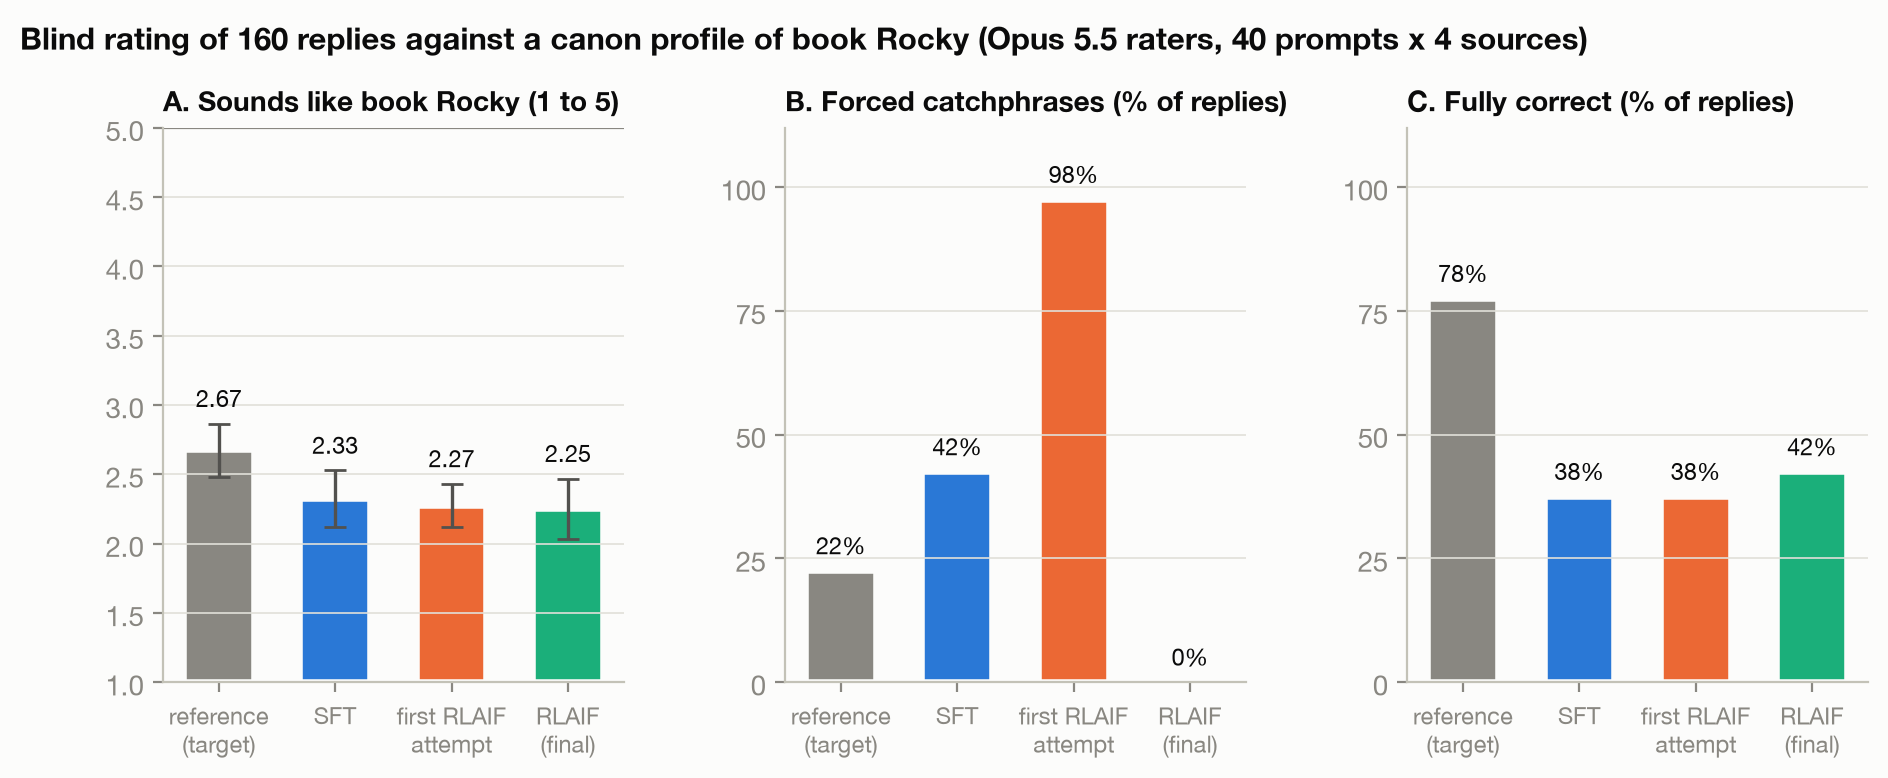
\includegraphics[width=0.9\textwidth]{fig4_blind_canon_rating.png}
\caption{Blind canon-grounded evaluation of 160 replies from four earlier sources. The
holistic 1-to-5 score does not separate the visibly gamed first RLAIF run from SFT; the
targeted forced-catchphrase flag does. Error bars in panel A are 95\% intervals.}
\label{fig:blind}
\end{figure*}

This evaluation has substantial limitations. The canon rater is itself a model, each
reply is scored by only one of two rater instances, the human sample has four replies per
source, and only non-code prompts are rated. More fundamentally, the rewrite prompt
teaches habits that are weakly grounded in the novel: for example, ``Listen. Listen.''
is frequent in the training target, while the book-derived profile does not support it.
All automatic style scores can therefore reward fidelity to a synthetic target that is
not faithful to the character.

The project-authored five-dimension GPT-5.4 evaluation is complete for the earlier stages
but pending for the curriculum checkpoint. It uses the same style construct that informed
the training target, so model-provider separation does not make it fully independent.
We will report its dimensions separately,
leading with human plausibility rather than the ``markers'' dimension, which can reward
the same off-canon habits discussed above. Until that comparison is available, the
curriculum checkpoint is a provisional candidate, not a selected final model.
\clearpage

\section{Limitations and Threats to Validity}
\label{sec:limitations}

\paragraph{No replicated training runs.}
Each reported checkpoint comes from one training trajectory. We cannot separate method
effects from seed, sampling, or systems variance. Even greedy vLLM generations were not
bitwise repeatable in a repository check.

\paragraph{Checkpoint selection and repeated evaluation.}
The latest curriculum checkpoint is reported after inspecting benchmark trajectories.
Calling a point ``best'' is descriptive; it is not an unbiased held-out selection. A clean
confirmation would choose a checkpoint using training reward or a validation set and
evaluate the three test suites once.

\paragraph{Incomplete uncertainty.}
For 164-problem benchmarks, a single pass rate has a rough binomial uncertainty of
several percentage points. Stage comparisons are paired by problem, so a paired bootstrap
or McNemar analysis is preferable to independent binomial intervals. Those paired results
are not yet included.

\paragraph{Metric construction.}
Style cosine, centroid distance, catchphrase flags, and AI rubrics were all designed by
the project team. They are neither independent nor externally validated, and some target
the same markers used during training. The independent judge is also an AI system, not a
human ground truth.

\paragraph{Missing curriculum and data contamination.}
The run is described as excluding the named evaluation problems, but the exact 700-row
dataset and builder are absent. The committed 677-row file belongs to an older
MBPP/persona experiment and does not satisfy the current trainer's \texttt{test\_cases}
schema. We therefore cannot audit direct overlap, near duplicates across public code
corpora, or the base model's pretraining data.

\paragraph{Changing more than one variable.}
The failed and revised RLAIF runs differ in prompt, reward decomposition, learning rate,
and KL coefficient. Their contrast diagnoses a bad configuration but does not isolate
which change fixes it.

\section{Conclusion}

The experiment begins with a common post-training failure: SFT successfully installs a
surface persona while degrading a capability absent from most demonstrations. A naive
AI-judge objective then creates an obvious proxy exploit. Reward decomposition removes
that specific observed pattern, and the reported executable-reward curriculum recovers
much of the measured coding loss. The result does not establish that persona and coding
are generally compatible, nor that the latest checkpoint is preferable on every persona
measure. It does show why failure controls, disaggregated rewards, auditable data, a
separate final test, and multiple style metrics are necessary for making a credible claim.

\section*{Reproducibility Statement}

Training code, evaluation outputs, adapters, figure scripts, and this LaTeX source are
versioned in the project repository. Reproduction is incomplete: the latest 700-row
curriculum and its builder are missing, while the committed RLVR dataset is from an older
experiment and has an incompatible schema. The main result files are
\texttt{EVALS/results\_base}, \texttt{EVALS/results\_rlaif}, and the top-level files in
\texttt{EVALS/results\_rlvr}. Historical MBPP-based ablations are stored in named
subdirectories under \texttt{EVALS/results\_rlvr}. The paper figures are regenerated by
\texttt{report/scripts/fig\_*.py} and \texttt{RLVR/figures/plot\_rlvr.py}. The declared
Python environment also needs repair: its pinned Transformers version is incompatible
with the pinned sentence-transformers requirement. We therefore do not claim one-command
reproduction until the dataset and environment issues are fixed.

\balance
\bibliographystyle{plain}
\bibliography{references}

\end{document}
